\chapter{Introduction}
In this course, we will study the principles of modeling and analysis biology
data using simulation and AI models.

In the field of biology, the scale size varies from the organism like tree passing
through tissues and arriving at the cellular level. So we are considering elements
with the size that varies from meters to micrometers.

In particular, we can distinguish two main groups of organisms: bacteria and eukaryotes.

All this organisms have in common that all have DNA as genetic material. The DNA
is a molecule that contains the information necessary to build and maintain an
organism.

We can describe the DNA as a sequence of nucleotides. The nucleotides are the
building blocks of DNA. The DNA is a double helix structure, and the nucleotides
are paired in a specific way. The nucleotides are \textit{adenine}, \textit{thymine},
\textit{cytosine}, and \textit{guanine}.

This nucleotides are paired in the following way: \textit{adenine} with \textit{thymine}
and \textit{cytosine} with \textit{guanine}. This help us to save up space because
they are always complementary.

A \textbf{gene} is a sequence of nucleotides that contains the information to
create a protein. While a \textbf{genome} is the complete set of genes of an organism.

\begin{figure}[!ht]
    \centering
    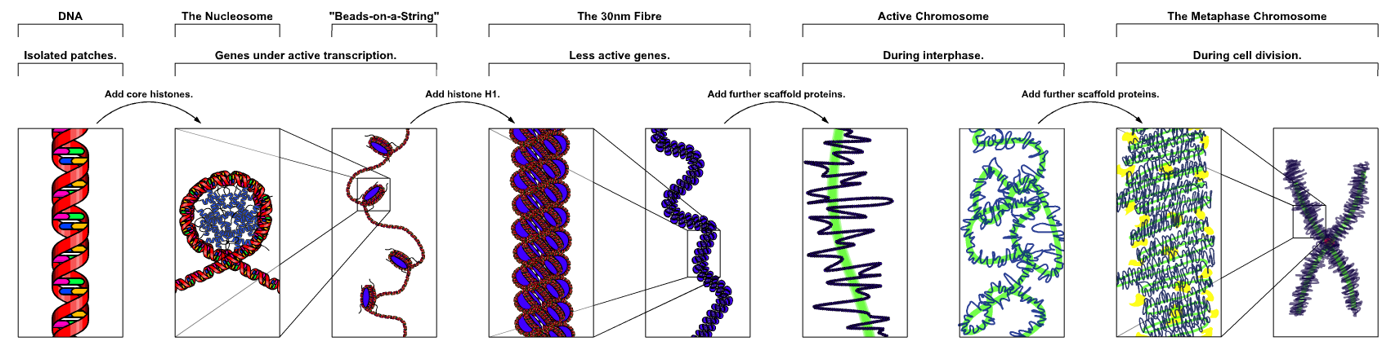
\includegraphics[width=\textwidth]{img/DNA.png}
    \caption{DNA structure}
    \label{fig:dna}
\end{figure}

A \textbf{genomic arm} refers to a large segment of a chromosome, typically
spanning several megabases (Mb) in size.

Starting from DNA we can create \textbf{RNA} through a process called \textbf{transcription}.
The RNA is a molecule that is used to create proteins. The proteins are the
building blocks of the cells. The process of creating proteins from RNA is called
\textbf{translation}.

The RNA transport information from nucleus, in other words, the DNA, to the
cytoplasm of a cell, where it mediates the process of translation to create proteins.

Once the information has passed into the protein it cannot get out again. The
transfer information from nucleic acid to nucleic acid, or from nucleic acid to
protein may be possible, but the transfer information from protein to protein,
or from protein to nucleic acid is impossible.
\section*{The Repressillator example}
A useful example to use as a base for the course is the repressillator. This is a
simple model of a genetic network that is able to oscillate. In particular, it is
compose of three proteins, $LacI$, $TetR$ and $\lambda CI$, that repress each other.

The structure of the repressillator is shown in Figure \ref{fig:repressillator}.
We can observe a circular structure, where each protein represses the next one in
the circle. This is a simple model of a genetic network that is able to oscillate.
More specifically, the LacI protein inhibits transcription of the second repressor
gene, TetR, which in turn inhibits the third repressor gene, $\lambda$ CI, which
in turn inhibits the first repressor gene, LacI.
\begin{figure}[!ht]
    \centering
    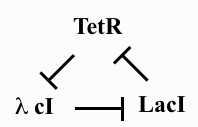
\includegraphics[width=0.5\textwidth]{img/repressillator.png}
    \caption{Structure of the repressillator.}
    \label{fig:repressillator}
\end{figure}

To implements this model, two \textbf{plasmids} are used. The plasmids are small
circular DNA molecules that are separate from the chromosomal DNA and can replicate
independently. The first plasmid codifies for the three proteins, while the second
plasmid serve as reporter of the system (GFP).

This system can be modeled using a set six of ordinary differential equations,
two for each protein. The general form of the equations is:
\begin{itemize}
    \item One equation for the variation of mRNA:
          \begin{equation}
              \frac{dM_i}{dt} = -m_i + \frac{\alpha}{1 + p_j^n} + \alpha_0
          \end{equation}
    \item One for representing the variation of the protein:
          \begin{equation}
              \frac{dP_i}{dt} = \beta (m_i - p_i)
          \end{equation}
\end{itemize}
where:
\begin{itemize}
    \item $\alpha$ is the proteins/cell from non repressed promoter.
    \item $\alpha_0$ is the proteins/cell from repressed promoter.
    \item $\beta$ protein mRNA decay velocity.
    \item $n$ Hill's coperativity coefficient.
\end{itemize}
\section{System, Biotech measures and Analysis}
During this course we want to measure two things:
\begin{itemize}
    \item \textbf{Gene expression}.
    \item \textbf{Gene alteration} also known as \textbf{mutation}.
\end{itemize}

The technology to obtain the information has evolved over time. In particular,
we have used \textit{microarrays} to measure gene expression, and now we use
\textit{next-generation sequencing} (NGS) for almost everything.

To collect data about gene expression, we can use \textbf{differential gene
    expression} (DGE). After using this approach, we can apply statistical
operation such as clustering or enrichment with genome ontology (GO).

With the enrichment phases we want to associate representative terms to the
clustering we have obtained. This operation is done in order to point out the
most important terms that are associated with the clustering.

\textbf{Gene ontology} is a controlled vocabulary that is use to describe gene.
It is divided in three categories:
\begin{itemize}
    \item \textbf{Biological process}: the biological objective to which the gene
          contributes.
    \item \textbf{Molecular function}: the biochemical activity of the gene product.
    \item \textbf{Cellular component}: the location of the gene product.
\end{itemize}
This information are express using a directed acyclic graph (DAG) where the main
type of association are \textbf{is a} and \textbf{part of}.
\subsection{Next-Generation Sequencing}
\textbf{Next-generation sequencing} (NGS) is a high-throughput methodology that
enables rapid sequencing of the base pairs in DNA or RNA samples.

The \textbf{sequencing} operation consists into fragmenting and extraction of
the DNA, then the DNA is sequenced and the \textbf{reads} are obtained. The reads
are short DNA fragments that are obtained from the sequencing process.

As computer scientists, we are interested in the dry-lab analysis which consists
in the \textbf{assembly} the \textit{reads} into a \textbf{Contigs}. Also, they
need to solve problem related to reads storage and allignments.

Talking about NGS, we can distinguish different approaches:
\begin{itemize}
    \item \textbf{Whole-genome sequencing} (WGS): the process of determining the
          complete DNA sequence of an organism's genome at a single time. This
          can be \textit{de novo} which mean that we don't have any reference
          genome.
    \item \textbf{Exome sequencing}: the process of capturing and sequencing the
          coding region of the genome.
    \item \textbf{Targeted sequencing}: the process of capturing and sequencing
          specific regions of the genome.
    \item \textbf{RNA sequencing} (RNA-Seq): the process of determining the
          complete RNA sequence of an organism's genome at a single time.
\end{itemize}

Also, talking about the analysis we can distinguish two types of analysis:
\begin{itemize}
    \item \textbf{Bulk analysis}: in this approach we use a pool of cells to analyze
          the gene expression. In particular, we create a average cell where we
          can study the overall gene expression.
    \item \textbf{Single cell analysis}: in this approach we analyze the gene
          expression of a single cell. This approach is more expensive and complex
          but it allows to study the gene expression of a single cell.
\end{itemize}
\subsection{From Sequencing to Mutational Information}
Thanks to the NGS we can obtain sequence that reveal different aspect of a
biological phenomenon. In this case, we can describe different subtypes of
mutations. Also, using bulk sequencing we can build a phylogeny tree that
describe the evolution of the mutation.